\documentclass[border=8pt]{standalone}
\usepackage[utf8]{inputenc}
\usepackage{tikz}
\usetikzlibrary{positioning}

\tikzset{
  debole/.style = {rectangle, draw, thick, fill=blue!8, double, double distance=1.5pt, minimum width=26mm, minimum height=16mm, font=\small},
  attr/.style   = {circle, draw, thick, fill=white, minimum size=5pt, inner sep=0},
  pk/.style     = {circle, draw, thick, fill=black, minimum size=5pt, inner sep=0},
  link/.style   = {thick},
  et/.style     = {font=\footnotesize}
}

\begin{document}
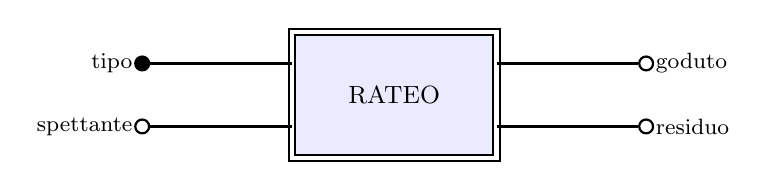
\begin{tikzpicture}
  \node[debole] (E) {RATEO};
  \node[pk]   (t) at (-3.2, 0.4){}; \draw[link] (-1.3, 0.4)--(t); \node[et,left] at (t) {tipo};
  \node[attr] (s) at (-3.2,-0.4){}; \draw[link] (-1.3,-0.4)--(s); \node[et,left] at (s) {spettante};
  \node[attr] (g) at ( 3.2, 0.4){}; \draw[link] ( 1.3, 0.4)--(g); \node[et,right] at (g) {goduto};
  \node[attr] (r) at ( 3.2,-0.4){}; \draw[link] ( 1.3,-0.4)--(r); \node[et,right] at (r) {residuo};
\end{tikzpicture}
\end{document}
